Рассмотрим задачу Коши для неоднородного уравнения колебаний
\[
	\derp{u}{t}{2} = a^2 \derp{u}{x}{2} + h(x, t)
\]
\[
		-\infty < x < \infty,	\quad	t > 0
\]
Начальные условия:
\begin{alignat*}{1}
	u(x, 0) &= f(x)\\
	\derp{u}{t}{} (x, 0) &= g(x)
\end{alignat*}

\begin{figure}[h!] 
	\centering 
	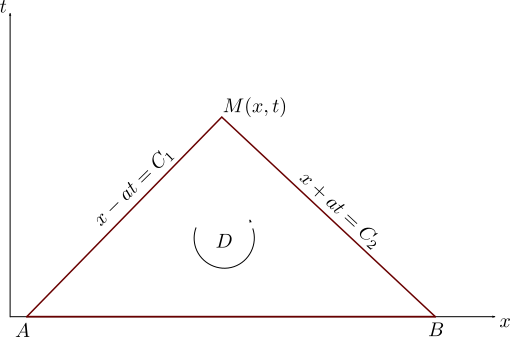
\includegraphics[width=0.6\textwidth]{figStringKoshi.pdf}
	\caption{Характеристический треугольник}
\end{figure}
Проинтегрируем обе части уравнения по области, заключённой внутри характеристического треугольника и разделим обе части на $2 a$.
\[
	\frac{1}{2a} \iint\limits_D \derp{u}{t}{2} dx dt = \frac{a}{2} \iint\limits_D \derp{u}{x}{2} dx dt + \frac{1}{2 a} \iint\limits_D h(x, t) dx dt
\]
Вспомним формулу Эйлера, которая помогает заменить интеграл по области на интеграл по границе.
По формуле Грина 
\[
	\iint\limits_D \derp{u}{t}{2} dxdt = - \oint\limits_{\partial D} \derp{u}{x}{} dt \qquad \iint\limits_D \derp{u}{x}{2} dx dt = \oint\limits_{\partial D} \derp{u}{x}{} dt
\]
\[
	- \oint_{\partial D} \derp{u}{t}{} = - \left[ \int\limits_A^B \derp{u}{t}{} dx + \int\limits_B^M \derp{u}{t}{} dx + \int\limits_M^A \derp{u}{t}{} dx \right] = 
\]
\[ 
	= - \int\limits_A^B \derp{u}{t}{} dx + a \int\limits_B^M \derp{u}{t}{} dt - a \int\limits_M^A \derp{u}{t}{} dt = 
\]
\[ 
	= - \int\limits_A^B \derp{u}{t}{} dx + 2 a u(M) - a u(A) - a u(B)
\]
\begin{multline*}
	\oint_{\partial D} \derp{u}{x}{} dt = \cancelto{0}{\int\limits_A^B \derp{u}{x}{} dt} + \int\limits_B^M \derp{u}{x}{} dt + \int\limits_M^A \derp{u}{x}{} dt = - \frac{1}{a} \int\limits_B^M \derp{u}{x}{} dx + \frac{1}{a} \int\limits_M^A \derp{u}{x}{} dx = \\ 
	=- \frac{2}{a} u(M) + \frac{(u(A) +u(B))}{a} = \frac{1}{2 a} \int\limits_A^B \derp{u}{t}{} dx + u(m) - \frac{u(B) +u(A)}{2} =\\=
	 - u(M) + \frac{u(B)+u(A)}{2}  + \frac{1}{2a} \iint\limits_D h(x, t) dx dt
\end{multline*}
\[
	2 u(M) = \frac{1}{2a} \int\limits_A^B \derp{u}{t}{} dx + u(A) +u(B) + \frac{1}{2a} \iint\limits_D h(x, t) dx dt
\]
\[
	x_m - at_m = C_1 = x - at \Rightarrow x_A = x_m - at_m
\]
\[
	x_m + at_m = C_2 = x + at \Rightarrow x_B = x_m - at_m
\]
Получим:
\[
	u(M) = \frac{u(x_m +at_m) + u(x_m - a t_m)}{2} + \frac{1}{2a} \int\limits_{x_m - at_m}^{x_m + a t_m} g(\xi) d \xi + \frac{1}{2a} \iint\limits_D h(x, t) dx dt
\]



